%
\documentclass[11pt]{article}
\usepackage{amssymb}
\usepackage{amsmath}
\usepackage{pst-all}
\usepackage{newicktree}
\usepackage{graphicx}
\usepackage[left=1.4in,right=1.4in,top=1in,bottom=1in,includeheadfoot]{geometry}
\usepackage{setspace}

\newtheorem{theorem}{Theorem}

\frenchspacing
\linespread{1.25}
\parskip= 2 pt

\title{Theoretical Foundations of the Age-Area Hypothesis}
\author{\textbf{Matthew J. Baker} \\ Department of Economics \\ Hunter College and the Graduate Center, CUNY}

\begin{document}

\maketitle
\begin{abstract}
\noindent The impact of past mass migrations is still felt today. One tool commonly used in theorizing about the nature and origins of mass migrations is the so-called Age-Area Hypothesis, originally advanced by Sapir (1915). The age-area hypothesis traces the origins of linguistic stocks, which are closely related to cultural and genetic similarities. One common way of stating the hypothesis
is that the area of origin of a linguistic stock is where the languages comprising the stock are most different. While the hypothesis is compelling, and its predictions are often corroborated by other evidence, a cohesive theoretical structure for the Age-Area Hypothesis has never been described. This paper describes such a theoretical foundation in terms of probability, and also presents a computational algorithm for computing the relative likelihood of historical locations and migratory paths.
\end{abstract}
\newpage

The age-area hypothesis - evidently first developed and applied by Sapir (1916) in his study of certain Native American Languages - is often invoked when linguistic
evidence is used in support of hypotheses about where different sorts of cultures originated, how they evolved over time, and how they came to be located where they are today. Briefly stated, the hypothesis says that the geographic area where a language phylogeny originated is most likely the place where the component languages of the phylogeny are maximally differentiated.



While the question may some of academic interest only, a wide variety of recent economic literature highlights the importance of understanding how we arrived at the current cultural mix around the globe. Coincident with this understanding is the realization that understanding where different cultures came from, and how they interacted in the past, is also of paramount importance.

Examples of the application of the linguistic age-area hypothesis  abound. Sapir himself used these arguments to suggest that the so-called Na-Dene linguistic grouping originated in and around the North West Coast. As another example, Atkinson and Gray (2003) have used the results to suggest that the Indo-European languages originated in Anatolia, not, as is sometimes supposed, on the steppes of Siberia. Further applications of the idea - either implicit or explicit use of the idea - are almost too numerous to mention. Ruhlen (2001) uses the age-area hypothesis to lend insight into debates about the origins of the Na-Dene, as well as the origins of the Bantu linguistic group in Africa.

What is the existing theoretical basis for the age-area hypothesis? In spite of its wide range of applications and deep implications for human history, there is almost no theoretical support for the hypothesis. In population genetics, it is well-known that
the point of maximal genetic diversity of populations is closest to the geographical point of origin. This is because migrant populations are subsets of the parent population, and hence have only a subset of the population genes. But this is certainly not the case with language; migrant populations don't migrate with only a subset of the vocabulary or grammar of the parent language! 

The lack of a theoretical basis for the  age area hypothesis is also a problem for its use in technical situations. For example, suppose one wished to include an ancient migratory path in a statistical model? Since the hypothesis has no theoretical underpinnings, it is difficult to see how to construct a likelihood for a certain path or migratory history.

In this paper, I develop a theoretical foundation for the age-area hypothesis, and make some of the terms supporting the hypothesis more rigorous. The theory is based upon a particular idea that turns out to correspond with a probabilistic notion of parsimony. The probablistic foundations, it turns out, can also be grounded in a particular type of shock that incites migration but then stochastically reverts to previous conditions. 

Finally, using the aforementioned methods, I develop an Age-Area Theorem, which says that a culture that is more distance linguistically from the others in the stock is also more likely to be the point of origin of the stock. 
\section{Problem Description and Motivation}

Consider the hypothetical phylogenetic tree displayed in figure \ref{fig1}. The figure depicts the genetic relationship between five related cultures.  In the usual lingo, A is the `most divergent,' with B, C, D, E all being more closely related. D and E are the most closely related cultures. To avoid forming impressions based on evidence that is not part of the hypothesis, we will suppose that the locations of the
groups have been concealed from us, and that we have no access to archaeological or historical information about the language stock.

The Age-Area hypothesis (henceforth the AAH) concerns the location in which this group of societies originated, and the times and sequences behind how they subsequently migrated to populate their current locations. The AAH posits that the point of origin was A's location, as A is the most divergent language from the group. If one wanted to push the hypothesis a bit further, or even apply it recursively, one would come up with a hypothetical migratory route: the hypothesis would lead one to believe that the point of origin of the stock was A, at which point there was a migration from A to B, then from B to C, and then from C to either D or E.

\begin{figure}
\begin{center}
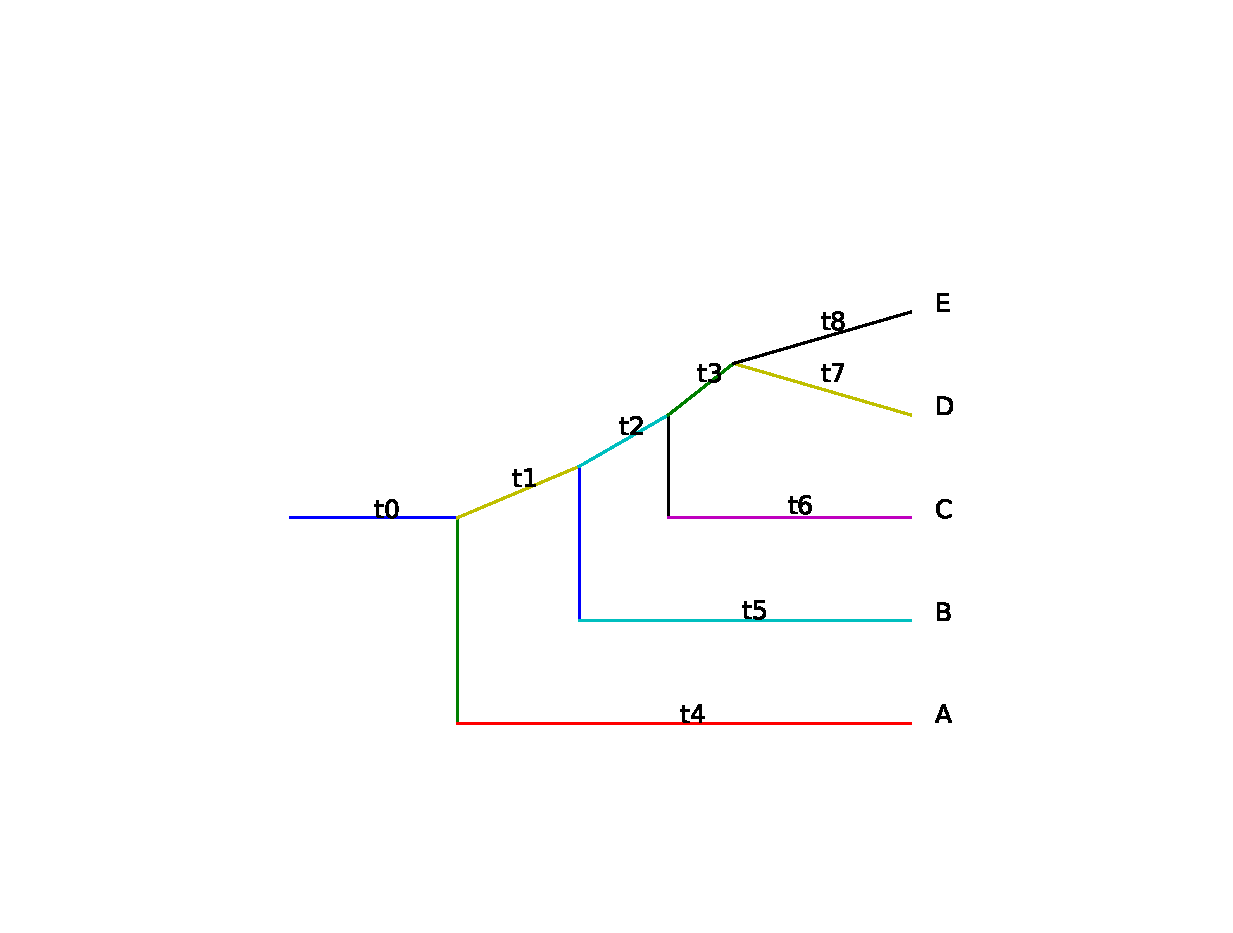
\includegraphics[width=\textwidth]{simplePT.eps}
\caption{A simple phylogenetic tree} \label{fig1}
\end{center} 
\end{figure}

There are a large number of other possibilities as well, even though the structure of the tree constrains some sorts of events. For example, an additional plausible sequence of migratory events would be for an initial migratory episode from C to A, followed by another from C to B, followed by yet another migration from C to D or E.

\begin{figure}
\begin{center} 
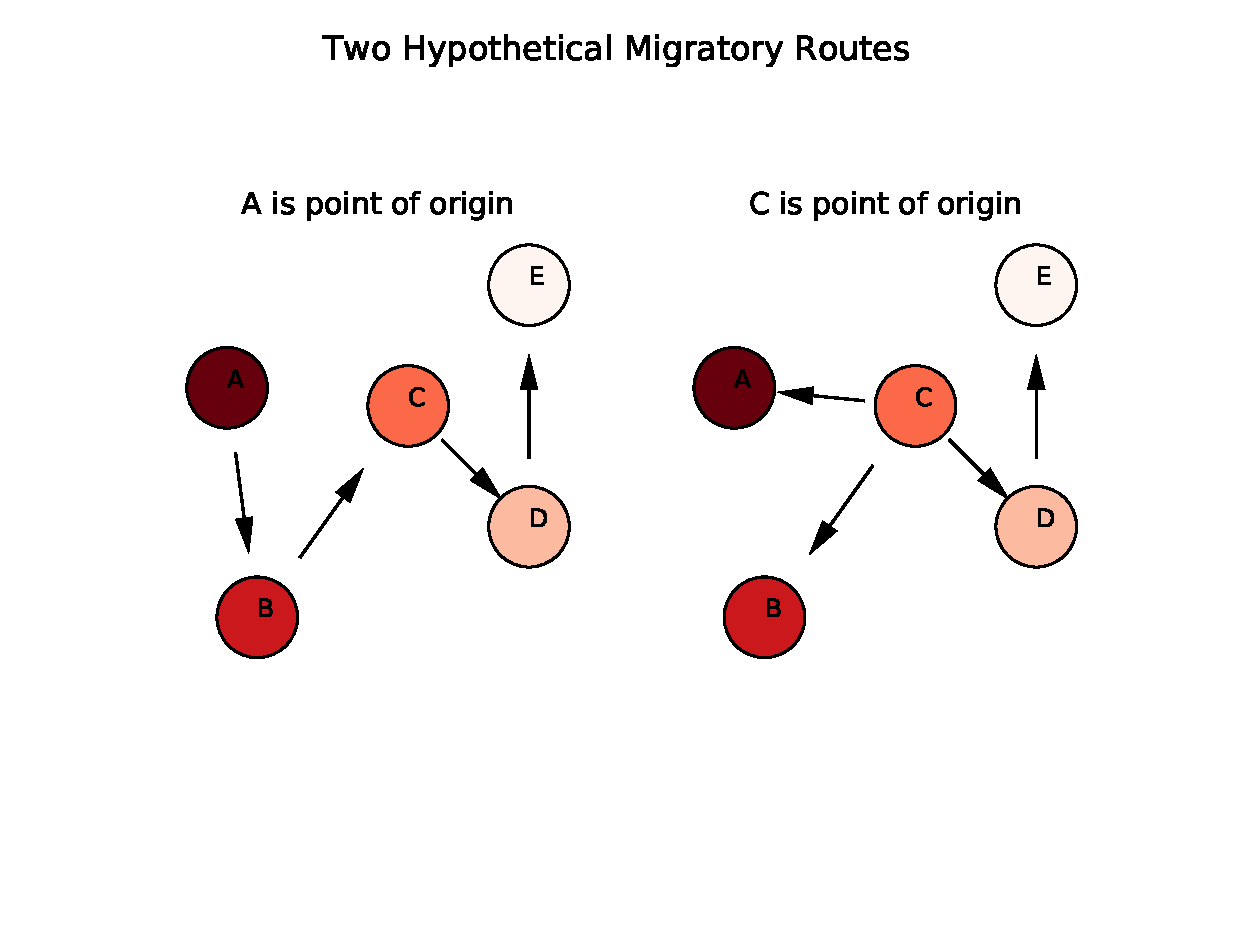
\includegraphics[width=\textwidth]{simpleMR.eps} 
\caption{Potential migratory routes among a language stock consisting of five groups, following the Phylogenetic Tree in figure.} \label{fig2}
\end{center} 
\end{figure}

These two possible migratory routes are presented in figure \ref{fig2}. The AAH suggests that the second sequence is a less likely migratory history than the sequence. Why? For a variety of reasons - one might simply appeal to Occam's razor - the events on the left-hand side of figure \ref{fig2} require only one migratory chain, while the events on the right-hand side require three separate expansions: an initial migration from A to C, followed by another from A to B. A third migratory event is sufficient to take care of the last two groups: it begins from C continues to D, and then to E. We can now pose our question as follows: if we believe these migratory events to be rare, and we wish to conserve them in explaining historical migrations, what sort of model would accomplish this? But can one make this operational in a more formal setting? Can one characterize parsimony in a meaningful mathematical and probabilistic way? 

\section{A model}

In addition to providing a foundation for the age-area hypothesis, we might lean on some additional principles that we wish to encapsulate in the theory. We might like the model to conserve on estimation of parameters, and we might also like the model to have a consistent internal logic. A simple model with transparent machinery also creates the possibility of expansion and further development. While the assumptions listed below are restrictive, one can see how they might be relaxed in future work. 

Along these lines, assume that we observe the entire phylogenetic tree, and that there are no unobserved migratory events. The tree is assumed to be a full, rooted, binary tree, meaning that there is a single origin node and branch, and all other nodes have a single parent. All the interior nodes have two children, and all terminal nodes (leaves) have zero children. Figure \ref{fig2} is an example of such a tree.  

We flesh out a model of migration following definition of a migratory chain. 
\begin{enumerate}
\item Migratory chains are unique in the sense that each is governed by its own parameters. 
\item  A migratory chain can begin with any location that is currently occupied. \item The location where the chain appeared generates a mass-migration at time $t$ according to an exponential distribution with parameter $\lambda$.
\item The group emitting the mass-migration also loses its propensity to migrate. This propensity to migrate is carried off with the mass-migrating group to its new location. 
\end{enumerate}

One good thing about this model is that it can be easily concentrated, and also easily expanded or contracted depending on the evidence available the researcher. In some situations, for example, one has information about the exact times at which splits have occurred. If times are known, one can use an exponential distribution to govern the splits, while if times are not known, one can use a Poisson distribution. In either case, the parameters of the model can be concentrated to leave a simple probability that the observed culture group originated at each point. 

In other instances, one might learn know the structure of the tree but not the exact times at which events have occurred. That is, the parameters of any exponential distribution can be concentrated out of the likelihood, and this makes the workings of the model clear in that one can easily see how and why it would posit that the first sequence of events on figure \ref{fig2} are more likely.

To see the basic idea, let's develop a comparison of the two scenarios described in figure \ref{fig2}. The first scenario requires an initial migratory event to start after time $t_0$ from point $A$. At this point, according to the model assumptions, $A$ is dormant, and the migratory bug is transitioned to location $B$. After time $t_1$, $B$ emits the migratory bug to $C$ and is then dormant, followed by $C$'s emission and subsequent dormancy, and then $D$'s. Finally, $E$ retains the bug but never emits.

This is the only migratory episode needed to explain the positioning of the groups in the tree, and given the assumption that discharges are exponential, suppose our events are described by the distribution $\textrm{Exp}(\lambda)$. Then, we have the likelihood of point $A$ being the point of origin as:
\begin{equation} \label{e1}
P_A = \lambda e^{-\lambda t_0}\lambda e^{-\lambda t_1}\lambda e^{-\lambda t_2}\lambda e^{-\lambda t_3}e^{-\lambda t_8}
\end{equation}
or
\begin{equation} \label{e2}
P_A = \lambda^4 e^{-\lambda (t_0+t_1+t_2+t_3+t_8)}
\end{equation}

There are a couple of points of interest for equation (\ref{e1}). First, since only one migratory path is needed to explain the events, only one
exponential parameter is needed for the whole process. Also, since a migratory event after $t_8$ is never observed, we have $1-F(t_8,\lambda) = e^{-\lambda t_8}$; there is only one such ``operational branch'' when our observation period ends.

Since the migration parameter is not of as great of interest as the probability, we can take the log of equation $\ref{e2}$ and maximize the result with respect to $\lambda$, and substitute the result back in to concentrated likelihood, giving us a closed-form expression for the probability that $A$ is the point of origin:
\begin{equation} \label{e2}
P_A = \frac{4^4e^{-4}}{(t_0+t_1+t_2+t_3+t_8)^4}
\end{equation}
Of course, this is not all that meaningful without a point of comparison. So, by way of comparison, according to this model, what is the likelihood that the point of origin is $C$?

In this case, the process begins with a migration after $t_0$ from $C$ to $A$. Subsequently, no additional migrations occur from $A$, so $A$ remains active. Then, after time $t_1$ a second migratory event arises leading from $C$ to $B$, after which nothing further occurs on this branch. Then, a migratory event leads from $C$ to $D$ over time $t_2$, and then from $D$ to $E$ over time $t_3$, at which point nothing more happens.

The key thing about this explanation is that there are three separate migratory events needed to explain things, so we need three exponential parameters in the model. Another key thing is that we have more branches that are ``alive'' at the end of the process. These might suggest intuitively that this explanation is less likely than the previous, and this is indeed the case under the model. Forming the likelihood in the
same way as we did above, we have:
\begin{equation} \label{e3}
P_C = \lambda_1e^{-\lambda_1(t_0+t_4)} \lambda_2 e^{-\lambda_2 (t_1+t_5)}\lambda_3^2 e^{-\lambda_3 (t_2+t_3+t_8)}
\end{equation}
So, here we have a three-parameter model, which is how the increased complexity of the explanation (the anti-Occam's razor effect) is manifest in the probability. Concentrating \ref{e3} as above gives the result:
\begin{equation} \label{e4}
\frac{2^2e^{-4}}{(t_0+t_4)(t_1+t_5)(t_2+t_3+t_5)}
\end{equation}

 We can form the ratio of this and the previous expression and see which tree is more likely under which configuration of the parameters. The intuition behind the explanation can be written as:
 \begin{equation*}
 LR = 4\left({1-\frac{t_0}{T}}\right)4^2\left(1-\frac{t_o+t_1}{T}\right)^2
 \end{equation*}
So we see that unless the branches $t_0$ and $t_1$ constitute a (very) large span of the tree, our model claims that $A$ is the most likely place of origin.

\section{Theorems}

\begin{theorem}{The Age-Area theorem}

Take the route collection $R$ through tree $T$ and apply to it a redirect, calling the result $R'$. Then, compute the concentrated likelihood of the new tree gives $p(R) > p(R')$. 
\end{theorem}


\section{An algorithm}

As is often the case when dealing with estimation over trees, it behooves one to consider an algorithm that works backwards from the branches to the base. The algorithm presented here is essentially a pruning algorithm like Felsenstein's with a hint of dynamic programming. The dynamic programming aspect introduces a sort of continuation maximum likelihood into the tree.

The algorithm works as follows. At termination, the result is a concentrated log-likelihood of each location being the point of origin.  The following is an illustration showing how the algorithm works on the example given above.

\begin{enumerate}
\item[0.] Initialization: a ``active'' vector of zeros $A=[0,0,0,0,0]$, a vector of exponential parameters that start with zero, $E=[0,0,0,0,0]$, and a continuation likelihood $L=[-t_4,-t_5,-t_6,-t_7,-t_8]$
\item  Select an interior node and pick out its branches.
\item  Poo I\ can add stuff again! \end{enumerate}

\cite{gildner91}
\cite{dowd09}





\bibliographystyle{apalike}
\bibliography{bibfile}

\end{document} 
